\section*{Structure of exam \modulecode}
The general shape of a theoretical exam for \texttt{\modulecode} is made up of highly structured open questions.

\paragraph{Question 1: } \ \\

\textbf{General shape of the question:} \textit{Given the following class definitions, and a piece of code that uses them, fill in the stack, heap, and PC with all steps taken by the program at runtime.}

\textbf{Concrete example of question:}

\lstset{numbers=left,basicstyle=\ttfamily\small}\lstset{language=[Sharp]C}
\begin{lstlisting}
public interface Option<T>
{

  U Visit<U>(Func<U> onNone, Func<T, U> onSome);
}
public class Some<T> : Option<T>
{
  T value;
  public Some(T value) { this.value = value; }
  public U Visit<U>(Func<U> onNone, Func<T, U> onSome)
  {
    return onSome(value);
  }
}
public class None<T> : Option<T>
{
  public U Visit<U>(Func<U> onNone, Func<T, U> onSome)
  {
    return onNone();
  }
}
...
Option<int> number = new Some<int>(5);
int inc_number = number.Visit(() => { throw new Exception("Expecting a value..."); }, i => i + 1);
Console.WriteLine(inc_number);
\end{lstlisting}
\textbf{Points:} \textit{3 (30\% of total).}

\textbf{Grading:} \textit{one point per correctly filled-in execution step.}

\textbf{Associated learning objective:} \glsfirst{abs}

\ \\ 

\paragraph{Question 2: } \ \\

\textbf{General shape of question:} \textit{Given the following class definitions, and a piece of code that uses them, fill in the declarations, class definitions, and PC with all steps taken by the compiler while type checking.}

\textbf{Concrete example of question:} 

\lstset{numbers=left,basicstyle=\ttfamily\small}\lstset{language=[Sharp]C}
\begin{lstlisting}
public interface Option<T>
{
  U Visit<U>(Func<U> onNone, Func<T, U> onSome);
}
public class Some<T> : Option<T>
{
  T value;
  public Some(T value) { this.value = value; }
  public U Visit<U>(Func<U> onNone, Func<T, U> onSome)
  {
    return onSome(value);
  }
}
public class None<T> : Option<T>
{
  public U Visit<U>(Func<U> onNone, Func<T, U> onSome)
  {
    return onNone();
  }
}
...
Option<int> number = new Some<int>(5);
int inc_number = number.Visit(() => { throw new Exception("Expecting a value..."); }, i => i + 1);
Console.WriteLine(inc_number);
\end{lstlisting}

\textbf{Points:} \textit{3 (30\% of total).}

\textbf{Grading:} \textit{Grading: one point per correctly filled-in type checking step.}

\textbf{Associated learning objective:} \glsfirst{type}

\paragraph{Question 3: }

\textbf{General shape of question:} \textit{Given the following UML diagram of a design pattern, fill in the missing parts.}

\textbf{Concrete example of question:} 

\begin{center}
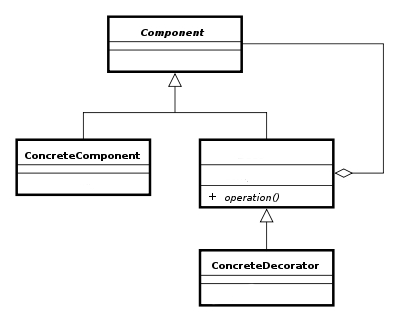
\includegraphics[width=\textwidth / 2]{decorator_uml}
\end{center}

\textbf{Points:} \textit{4 (40\% of total).}

\textbf{Grading:} \textit{Grading: one point per correctly filled-in block of code.}

\textbf{Associated learning objective:} \glsfirst{abs}

\ \\
